\documentclass[a4paper,12]{article}
\usepackage{amsmath, amsfonts, amssymb, amsthm, bm, graphics, bbm, color}
\usepackage{graphicx}
\usepackage{subfigure}
\usepackage{mathtools}
\usepackage[table]{xcolor}
\usepackage{url}
\usepackage{mathabx}
\usepackage{cancel}
\usepackage{multicol}
\usepackage{float}
\usepackage{caption}
\usepackage{mathalfa}
\usepackage{hyperref}
\usepackage{afterpage}
\usepackage{multirow}
\usepackage[section]{placeins}

\captionsetup{font=footnotesize}
\captionsetup{width=\textwidth}
\DeclareMathAlphabet\mathbfcal{OMS}{cmsy}{b}{n}
\newtheorem{theorem}{Theorem}[section]
\newtheorem{lemma}[theorem]{Lemma}
\newtheorem{corollary}[theorem]{Corollary}
\newtheorem{proposition}[theorem]{Proposition}
\theoremstyle{definition}
\newtheorem{definition}[theorem]{Definition}
\newtheorem{example}[theorem]{Example}
\newtheorem{remark}[theorem]{Remark}


%center table entries
\newcolumntype{P}[1]{>{\centering\arraybackslash}p{#1}}


\newcommand\y{\cellcolor{gray!50}}

\newcommand\p{\cellcolor{gray!25}}

\makeatletter
\newcommand\makebig[2]{%
  \@xp\newcommand\@xp*\csname#1\endcsname{\bBigg@{#2}}%
  \@xp\newcommand\@xp*\csname#1l\endcsname{\@xp\mathopen\csname#1\endcsname}%
  \@xp\newcommand\@xp*\csname#1r\endcsname{\@xp\mathclose\csname#1\endcsname}%
}
\makeatother

\makebig{biggg} {3.0}
\makebig{Biggg} {3.5}
\makebig{bigggg}{4.0}
\makebig{Bigggg}{4.5}
\makebig{biggggg}{5.0}
\makebig{Biggggg}{5.5}
\makebig{bigggggg}{6.0}
\makebig{Bigggggg}{6.5}

\newcommand\bovermat[2]{%
    \makebox[0pt][l]{$\smash{\overbrace{\phantom{%
                    \begin{matrix}#2\end{matrix}}}^{\text{#1}}}$}#2}

\newcommand\bundermat[2]{%
    \makebox[0pt][l]{$\smash{\underbrace{\phantom{%
                    \begin{matrix}#2\end{matrix}}}_{\text{#1}}}$}#2}

\newcommand\partialphantom{\vphantom{\frac{\partial e_{P,M}}{\partial w_{1,1}}}}


\newcommand{\raisesym}[2]{\raisebox{0.5\depth}{$#1\Biggggg \}$}}

% redefine paper size
\setlength{\oddsidemargin}{0in}
\setlength{\textwidth}{6.4in}
\setlength{\topmargin}{-0.5in}
\setlength{\textheight}{9.9in}
\setlength{\headheight}{0in}

%slanted vector symbols
\renewcommand{\vec}[1]{\mbox{\boldmath$#1$}}
\newcommand{\vect}[1]{\boldsymbol{#1}}

%vertical d symbol for integrals
\newcommand{\dif}{\mathrm{d}}
\newcommand{\im}{\mathrm{i}}

\newcommand{\bbR}{\mathbb{R}}
\newcommand{\tr}{\mathrm{tr}}

\newcommand{\vvtheta}{{\bm {\vartheta}}}
\newcommand{\vvphi}{{\bm {\varphi}}}
\newcommand{\vtheta}{{\bm {\theta}}}


\DeclareMathOperator*{\esssup}{ess \, sup}

\begin{document}
\title{Angle measures for the measured Glock MPT characterisation}
%\author{P.D. Ledger}
\date{18th March 2024}
\maketitle
Notice how $\lambda_2(\tilde{\mathcal R})\approx \lambda_3(\tilde{\mathcal R})$ and $\lambda_2({\mathcal I})\approx \lambda_3({\mathcal I})$ for large $\omega$. When the eigenvalue curves become close (or cross each other) then this indicates the presence of eigenvalues with algebraic multiplicity greater than one.  The associated eigenvectors for an eigenvalue with algebraic multiplicity two 
 can be arbitrarily chosen as any two vectors that form a basis for the two-dimensional eigenspace. In numerical computations, the computation of eigenvectors associated with eigenvalues $\lambda_n , \lambda_m$ is problematic when $\lambda_n \to \lambda_m$. 

 Angles between the computed eigenvectors using the metrics $d_R$ and $d_F$ are considered and  the approximations $d_E$ and $d_C$ that do not require knowledge of the eigenvectors. Notice the smooth transition of   $d_R$ and $d_F$  in the regions where $\lambda_2(\tilde{\mathcal R})\approx \lambda_3(\tilde{\mathcal R})$ and $\lambda_2({\mathcal I})\approx \lambda_3({\mathcal I})$ and the associated {\bf peaks}.
While we know there are issues with the eigenvectors of repeated eigenvalues, the peaks are interesting as there is a {\bf smooth transition to them} and have not appeared in other simple objects that have been tested.
Also, while $d_E$ and $d_C$ do not capture the increase for large $\omega$ the normalising constant involved in the computation does identity an increase in this region. This is to be expected given the form the normalising constant  takes.


\begin{figure}[h]
\begin{center}
$\begin{array}{cc}
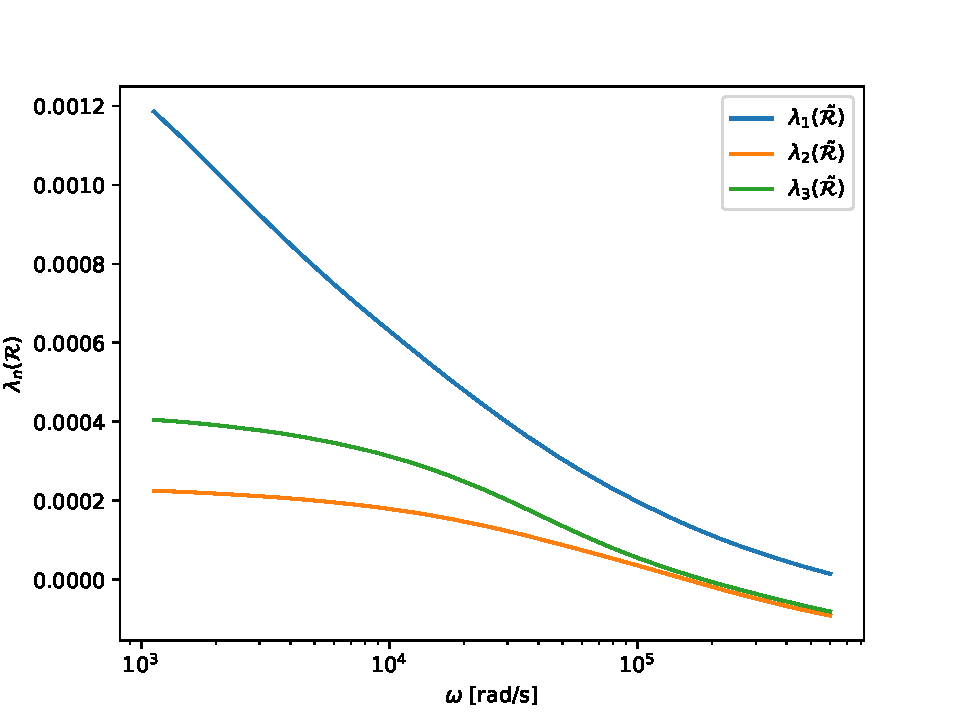
\includegraphics[width=0.5\textwidth]{glock_measured_RealEigenvalues.pdf} &
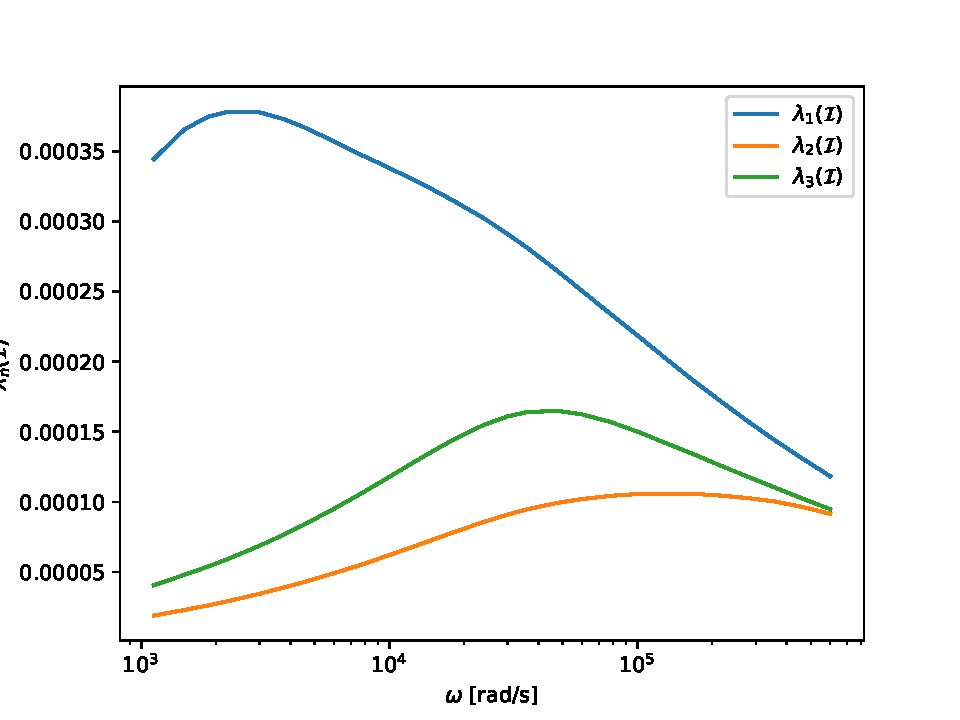
\includegraphics[width=0.5\textwidth]{glock_measured_ImaginaryEigenvalues.pdf}
\end{array}$
\end{center}
\caption{Measured $\lambda_n(\tilde{\mathcal R})$ (left) and  $\lambda_n({\mathcal I})$ (right) for the Glock object. Notice how $\lambda_2(\tilde{\mathcal R})\approx \lambda_3(\tilde{\mathcal R})$ and $\lambda_2({\mathcal I})\approx \lambda_3({\mathcal I})$ for large $\omega$}
\end{figure}

\begin{figure}[h]
\begin{center}
$\begin{array}{cc}
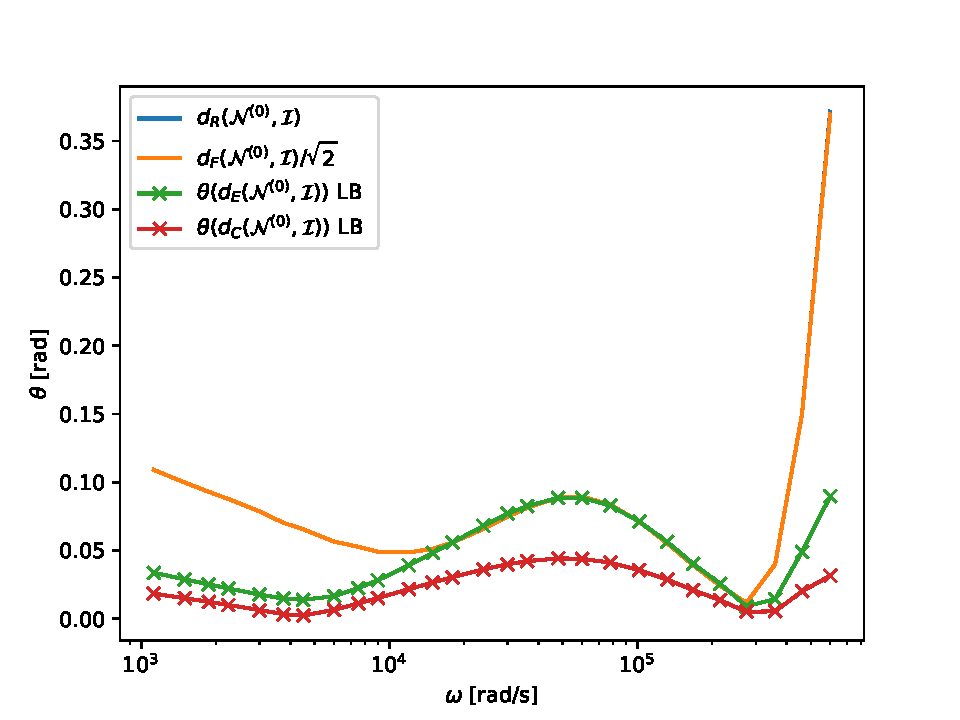
\includegraphics[width=0.5\textwidth]{glock_measured_N0I.pdf} &
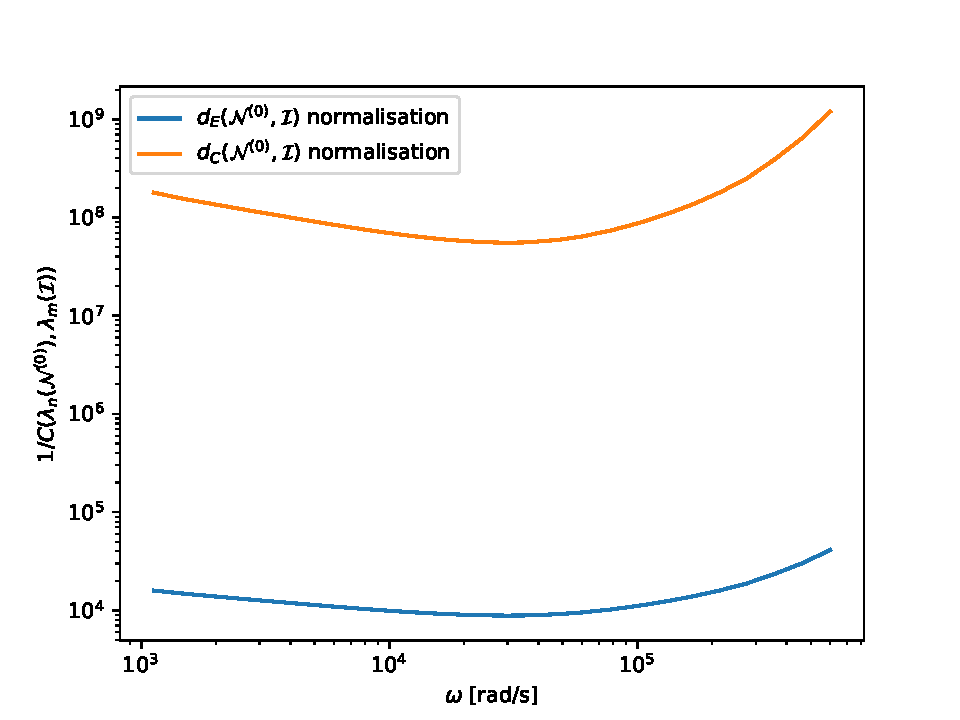
\includegraphics[width=0.5\textwidth]{glock_measured_N0I_den.pdf}
\end{array}$
\end{center}
\caption{Left: Angle measures $d_R({\mathcal N}^{(0)}, {\mathcal I})$ and $d_F({\mathcal N}^{(0)}, {\mathcal I})/\sqrt{2}$ using the eigenvectors and $\theta(d_E({\mathcal N}^{(0)}, {\mathcal I}) $ and $\theta(d_C({\mathcal N}^{(0)}, {\mathcal I} ) /\sqrt{2}$ without using the eigenvectors Right: Normalising constants in  $\theta(d_E({\mathcal N}^{(0)}, {\mathcal I}))$ and $\theta(d_C({\mathcal N}^{(0)}, {\mathcal I}))$}
\end{figure}

\begin{figure}[h]
\begin{center}
$\begin{array}{cc}
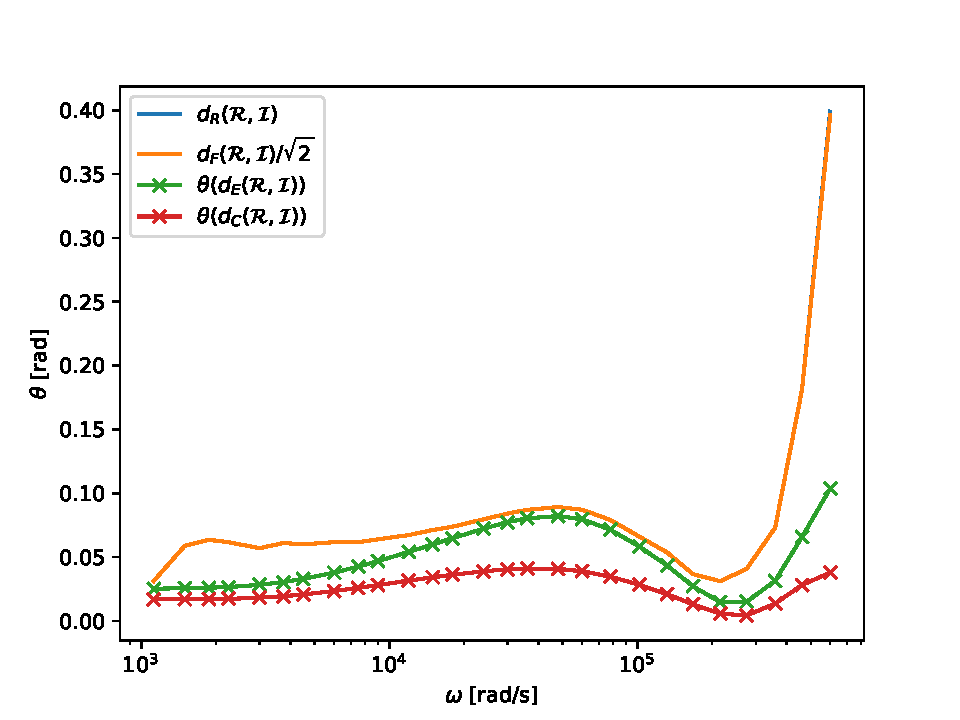
\includegraphics[width=0.5\textwidth]{glock_measured_RI.pdf} &
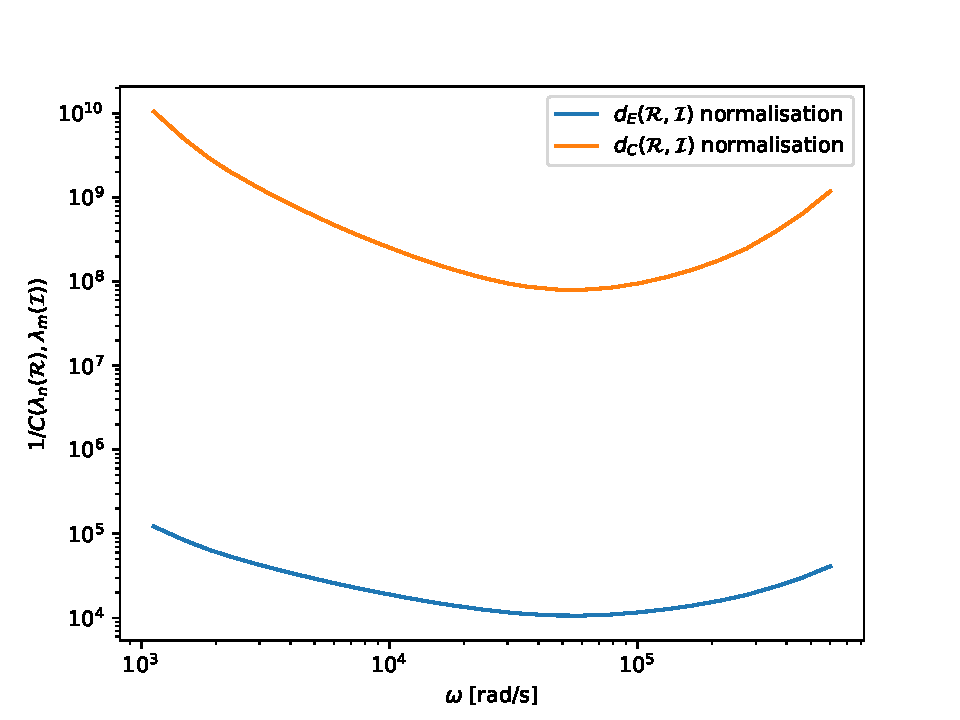
\includegraphics[width=0.5\textwidth]{glock_measured_RI_den.pdf}
\end{array}$
\end{center}
\caption{Left: Angle measures $d_R({\mathcal R}, {\mathcal I})$ and $d_F({\mathcal R}, {\mathcal I})/\sqrt{2}$ using the eigenvectors and $\theta(d_E({\mathcal R}, {\mathcal I}) $ and $\theta(d_C({\mathcal R} , {\mathcal I} ) $ without using the eigenvectors Right: Normalising constants in  $\theta(d_E({\mathcal R}, {\mathcal I}))$ and $\theta(d_C({\mathcal R}, {\mathcal I}))$}
\end{figure}

\begin{figure}[h]
\begin{center}
$\begin{array}{cc}
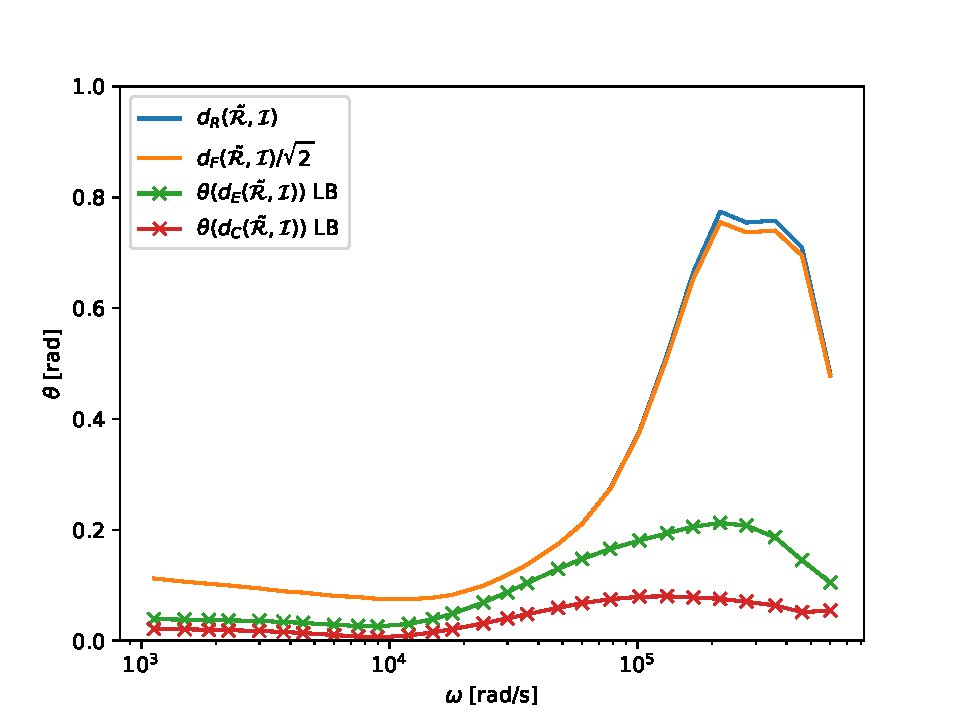
\includegraphics[width=0.5\textwidth]{glock_measured_RtildeI.pdf} &
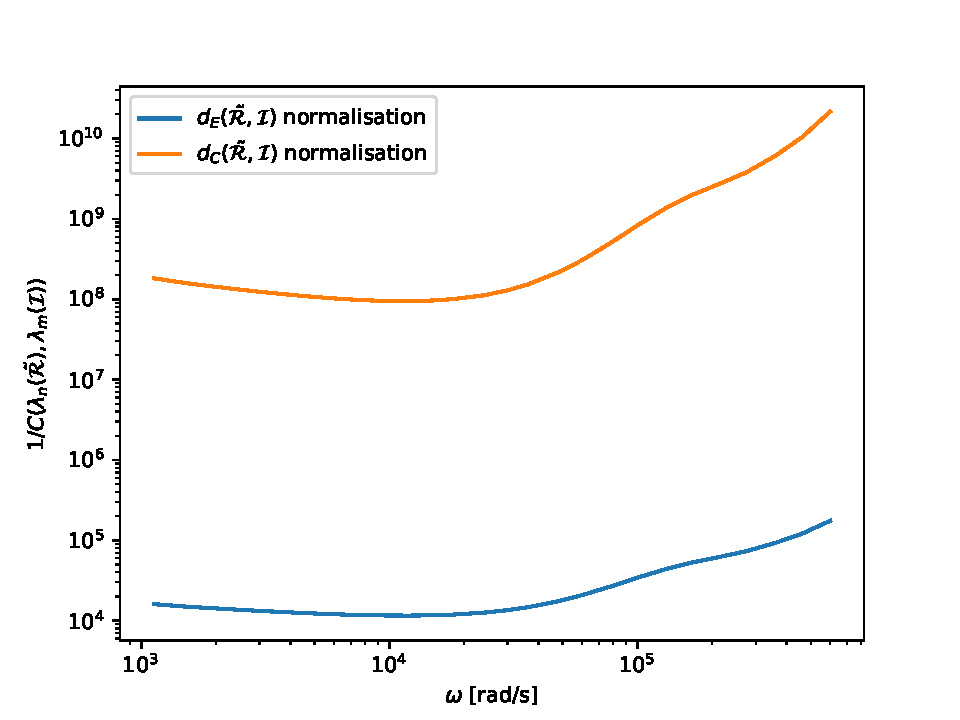
\includegraphics[width=0.5\textwidth]{glock_measured_RtildeI_den.pdf}
\end{array}$
\end{center}
\caption{Left: Angle measures $d_R(\tilde{\mathcal R}, {\mathcal I})$ and $d_F(\tilde{\mathcal R}, {\mathcal I})/\sqrt{2}$ using the eigenvectors and $\theta(d_E(\tilde{\mathcal R}, {\mathcal I}) $ and $\theta(d_C(\tilde{\mathcal R} , {\mathcal I} ) $ without using the eigenvectors Right: Normalising constants in  $\theta(d_E(\tilde{\mathcal R}, {\mathcal I}))$ and $\theta(d_C(\tilde{\mathcal R}, {\mathcal I}))$}
\end{figure}

\end{document}